%% 
%% Copyright 2007, 2008, 2009 Elsevier Ltd
%% 
%% This file is part of the 'Elsarticle Bundle'.
%% ---------------------------------------------
%% 
%% It may be distributed under the conditions of the LaTeX Project Public
%% License, either version 1.2 of this license or (at your option) any
%% later version.  The latest version of this license is in
%%    http://www.latex-project.org/lppl.txt
%% and version 1.2 or later is part of all distributions of LaTeX
%% version 1999/12/01 or later.
%% 
%% The list of all files belonging to the 'Elsarticle Bundle' is
%% given in the file `manifest.txt'.
%% 

%% Template article for Elsevier's document class `elsarticle'
%% with numbered style bibliographic references
%% SP 2008/03/01

\documentclass[preprint,12pt, a4paper]{elsarticle}

%% Use the option review to obtain double line spacing
%% \documentclass[authoryear,preprint,review,12pt]{elsarticle}

%% For including figures, graphicx.sty has been loaded in
%% elsarticle.cls. If you prefer to use the old commands
%% please give \usepackage{epsfig}

%% The amssymb package provides various useful mathematical symbols
\usepackage{amssymb}
\usepackage{hyperref}
\setlength{\parindent}{0pt}
%% The amsthm package provides extended theorem environments
%% \usepackage{amsthm}

%% The lineno packages adds line numbers. Start line numbering with
%% \begin{linenumbers}, end it with \end{linenumbers}. Or switch it on
%% for the whole article with \linenumbers.
%\usepackage{lineno}

% for quarto

\usepackage{fancyvrb}
\usepackage{framed}
\usepackage{calc}
\usepackage{tabularx}
\usepackage{booktabs}
\usepackage{longtable}
\usepackage{float}
\usepackage{hyperref}
\usepackage{lineno}
\usepackage{xcolor}

\providecommand{\tightlist}{%
  \setlength{\itemsep}{0pt}\setlength{\parskip}{0pt}}
  
\NewDocumentCommand\citeproctext{}{}
\NewDocumentCommand\citeproc{mm}{%
  \begingroup\def\citeproctext{#2}\cite{#1}\endgroup}
\makeatletter
 % allow citations to break across lines
 \let\@cite@ofmt\@firstofone
 % avoid brackets around text for \cite:
 \def\@biblabel#1{}
 \def\@cite#1#2{{#1\if@tempswa , #2\fi}}
\makeatother

\newlength{\cslhangindent}
\setlength{\cslhangindent}{1.5em}
\newlength{\csllabelwidth}
\setlength{\csllabelwidth}{3em}
\newenvironment{CSLReferences}[2] % #1 hanging-indent, #2 entry-spacing
 {\begin{list}{}{%
  \setlength{\itemindent}{0pt}
  \setlength{\leftmargin}{0pt}
  \setlength{\parsep}{0pt}
  % turn on hanging indent if param 1 is 1
  \ifodd #1
   \setlength{\leftmargin}{\cslhangindent}
   \setlength{\itemindent}{-1\cslhangindent}
  \fi
  % set entry spacing
  \setlength{\itemsep}{#2\baselineskip}}}
 {\end{list}}
\newcommand{\CSLBlock}[1]{\hfill\break#1\hfill\break}
\newcommand{\CSLLeftMargin}[1]{\parbox[t]{\csllabelwidth}{\strut#1\strut}}
\newcommand{\CSLRightInline}[1]{\parbox[t]{\linewidth - \csllabelwidth}{\strut#1\strut}}
\newcommand{\CSLIndent}[1]{\hspace{\cslhangindent}#1}

\newcommand{\VerbBar}{|}
\newcommand{\VERB}{\Verb[commandchars=\\\{\}]}
\DefineVerbatimEnvironment{Highlighting}{Verbatim}{commandchars=\\\{\}}
\definecolor{shadecolor}{RGB}{248,248,248}
\newenvironment{Shaded}{\begin{snugshade}}{\end{snugshade}}
\newcommand{\AlertTok}[1]{\textcolor[rgb]{0.94,0.16,0.16}{#1}}
\newcommand{\AnnotationTok}[1]{\textcolor[rgb]{0.56,0.35,0.01}{\textbf{\textit{#1}}}}
\newcommand{\AttributeTok}[1]{\textcolor[rgb]{0.77,0.63,0.00}{#1}}
\newcommand{\BaseNTok}[1]{\textcolor[rgb]{0.00,0.00,0.81}{#1}}
\newcommand{\BuiltInTok}[1]{#1}
\newcommand{\CharTok}[1]{\textcolor[rgb]{0.31,0.60,0.02}{#1}}
\newcommand{\CommentTok}[1]{\textcolor[rgb]{0.56,0.35,0.01}{\textit{#1}}}
\newcommand{\CommentVarTok}[1]{\textcolor[rgb]{0.56,0.35,0.01}{\textbf{\textit{#1}}}}
\newcommand{\ConstantTok}[1]{\textcolor[rgb]{0.00,0.00,0.00}{#1}}
\newcommand{\ControlFlowTok}[1]{\textcolor[rgb]{0.13,0.29,0.53}{\textbf{#1}}}
\newcommand{\DataTypeTok}[1]{\textcolor[rgb]{0.13,0.29,0.53}{#1}}
\newcommand{\DecValTok}[1]{\textcolor[rgb]{0.00,0.00,0.81}{#1}}
\newcommand{\DocumentationTok}[1]{\textcolor[rgb]{0.56,0.35,0.01}{\textbf{\textit{#1}}}}
\newcommand{\ErrorTok}[1]{\textcolor[rgb]{0.64,0.00,0.00}{\textbf{#1}}}
\newcommand{\ExtensionTok}[1]{#1}
\newcommand{\FloatTok}[1]{\textcolor[rgb]{0.00,0.00,0.81}{#1}}
\newcommand{\FunctionTok}[1]{\textcolor[rgb]{0.00,0.00,0.00}{#1}}
\newcommand{\ImportTok}[1]{#1}
\newcommand{\InformationTok}[1]{\textcolor[rgb]{0.56,0.35,0.01}{\textbf{\textit{#1}}}}
\newcommand{\KeywordTok}[1]{\textcolor[rgb]{0.13,0.29,0.53}{\textbf{#1}}}
\newcommand{\NormalTok}[1]{#1}
\newcommand{\OperatorTok}[1]{\textcolor[rgb]{0.81,0.36,0.00}{\textbf{#1}}}
\newcommand{\OtherTok}[1]{\textcolor[rgb]{0.56,0.35,0.01}{#1}}
\newcommand{\PreprocessorTok}[1]{\textcolor[rgb]{0.56,0.35,0.01}{\textit{#1}}}
\newcommand{\RegionMarkerTok}[1]{#1}
\newcommand{\SpecialCharTok}[1]{\textcolor[rgb]{0.00,0.00,0.00}{#1}}
\newcommand{\SpecialStringTok}[1]{\textcolor[rgb]{0.31,0.60,0.02}{#1}}
\newcommand{\StringTok}[1]{\textcolor[rgb]{0.31,0.60,0.02}{#1}}
\newcommand{\VariableTok}[1]{\textcolor[rgb]{0.00,0.00,0.00}{#1}}
\newcommand{\VerbatimStringTok}[1]{\textcolor[rgb]{0.31,0.60,0.02}{#1}}
\newcommand{\WarningTok}[1]{\textcolor[rgb]{0.56,0.35,0.01}{\textbf{\textit{#1}}}}

\usepackage{graphicx}
\makeatletter
\newsavebox\pandoc@box
\newcommand*\pandocbounded[1]{% scales image to fit in text height/width
  \sbox\pandoc@box{#1}%
  \Gscale@div\@tempa{\textheight}{\dimexpr\ht\pandoc@box+\dp\pandoc@box\relax}%
  \Gscale@div\@tempb{\linewidth}{\wd\pandoc@box}%
  \ifdim\@tempb\p@<\@tempa\p@\let\@tempa\@tempb\fi% select the smaller of both
  \ifdim\@tempa\p@<\p@\scalebox{\@tempa}{\usebox\pandoc@box}%
  \else\usebox{\pandoc@box}%
  \fi%
}
% Set default figure placement to htbp
\def\fps@figure{htbp}
\makeatother
%

\journal{SoftwareX}

\begin{document}
\renewcommand{\labelenumii}{\arabic{enumi}.\arabic{enumii}}

\begin{frontmatter}
% %--- INSTRUCTIONS TO BE DELETED OR COMMENTED BEFORE SUBMISSION 

%   {\large\textbf{SoftwareX article template Version 4 (November 2023)}}
%   Before you complete this template, a few important points to note:
%   \begin{itemize}
% \item	This template is for an original SoftwareX article. If you are submitting an update to a software article that has already been published, please use the Software Update Template found on the Guide for Authors page.
% \item	The format of a software article is very different to a traditional research article. To help you write yours, we have created this template. We will only consider software articles submitted using this template.
% \item	It is mandatory to publicly share the code/software referred to in your software article. You’ll find information on our software sharing criteria in the SoftwareX \href{https://www.elsevier.com/journals/softwarex/2352-7110/guide-for-authors}{Guide for Authors}.  
% \item	It’s important to consult the \href{https://www.elsevier.com/journals/softwarex/2352-7110/guide-for-authors}{Guide for Authors} when preparing your manuscript; it highlights mandatory requirements and is packed with useful advice.
% \end{itemize}
% %
% Still got questions?
% Email our editorial team at softwarex@elsevier.com.

% \textbf{Now you are ready to fill in the template below. As you complete each section, please carefully read the associated instructions. All sections are mandatory, unless marked optional.
% Once you have completed the template, delete these instructions. In addition, please delete the instructions in the template (the text written in italics).}
%--- END OF INSTRUCTIONS TO BE DELETED OR COMMENTED BEFORE SUBMISSION 
 
%% Title, authors and addresses

%% use the tnoteref command within \title for footnotes;
%% use the tnotetext command for theassociated footnote;
%% use the fnref command within \author or \address for footnotes;
%% use the fntext command for theassociated footnote;
%% use the corref command within \author for corresponding author footnotes;
%% use the cortext command for theassociated footnote;
%% use the ead command for the email address,
%% and the form \ead[url] for the home page:
%% \title{Title\tnoteref{label1}}
%% \tnotetext[label1]{}
%% \author{Name\corref{cor1}\fnref{label2}}
%% \ead{email address}
%% \ead[url]{home page}
%% \fntext[label2]{}
%% \cortext[cor1]{}
%% \address{Address\fnref{label3}}
%% \fntext[label3]{}

\title{cpp11armadillo: an R package to use the Armadillo C++ library}

%% use optional labels to link authors explicitly to addresses:
%% \author[label1,label2]{}
%% \address[label1]{}
%% \address[label2]{}

\author[label1]{Mauricio Vargas Sepulveda}
\author[label2]{Jonathan Schneider Malamud}
\address[label1]{University of Toronto, Munk School of Global Affairs
and Public Policy and Department of Political
Science, m.sepulveda@mail.utoronto.ca}
\address[label2]{University of Toronto, Department of Electrical and
Computer Engineering}

\begin{abstract}
%% Text of abstract 
\textit{This article introduces `cpp11armadillo', an R package that
integrates the highly efficient Armadillo C++ linear algebra library
with R through the `cpp11' interface. Designed to offer significant
performance improvements for computationally intensive tasks,
`cpp11armadillo' simplifies the process of integrating C++ code into R.
This package is particularly suited for R users requiring efficient
matrix operations, especially in cases where vectorization is not
possible. Our benchmarks demonstrate substantial speed gains over native
R functions and Rcpp-based setups.}
\end{abstract}

\begin{keyword}
%% keywords here, in the form: keyword \sep keyword
R, C++, Armadillo, linear algebra, benchmarking

%% PACS codes here, in the form: \PACS code \sep code

%% MSC codes here, in the form: \MSC code \sep code
%% or \MSC[2008] code \sep code (2000 is the default)

\end{keyword}

\end{frontmatter}

%\linenumbers

\section*{Metadata}
\label{}

\begin{table}[!h]
\begin{tabular}{|l|p{6.5cm}|p{6.5cm}|}
\hline
\textbf{Nr.} & \textbf{Code metadata description} & \textbf{Metadata} \\
\hline
C1 & Current code version & v0.4.0 \\
\hline
C2 & Permanent link to code/repository used for this code version & \url{https://github.com/pachadotdev/cpp11armadillo} \\
\hline
C4 & Legal Code License   & Apache License 2.0. \\
\hline
C5 & Code versioning system used & git \\
\hline
C6 & Software code languages, tools, and services used & C++, R. \\
\hline
C7 & Compilation requirements, operating environments \& dependencies & C++11 and R 4.0.0 at least. \\
\hline
C8 & If available Link to developer documentation/manual & \url{https://pacha.dev/cpp11armadillo/} \\
\hline
C9 & Support email for questions & m.sepulveda@mail.utoronto.ca \\
\hline
\end{tabular}
\caption{Code metadata (mandatory)}
\label{codeMetadata} 
\end{table}

\newpage

\section{Motivation and significance}\label{motivation-and-significance}

As R continues to grow in popularity for statistical computing and data
analysis, it can create bottlenecks when working with large datasets.
The need to interface with lower-level languages like C++ to bypass
these bottlenecks has led to the development of tools like `Rcpp'
{[}1{]}, and more recently, `cpp11' {[}2{]}.

`cpp11armadillo' is a novel package that builds upon the existing
Armadillo C++ library {[}3{]} to provide high-level access to efficient
linear algebra operations directly from R. The existing `RcppArmadillo'
{[}4{]} already offers this, and `cpp11armadillo' offers an alternative
with modern C++ features, where we highlight vendoring, which can
improve performance and simplify the its usage.

This package is not designed for the average R user. Instead, it is
intended for users in academia or industry who require intensive linear
algebra computations. `cpp11armadillo' provides tools to bridge the gap
between ease of use and the computational efficiency demanded by such
workloads.

`RcppArmadillo' is a popular package for this purpose, it has existed
for nearly a decade, `cpp11armadillo' offers a different approach with
similar performance. Rewriting code from `RcppArmadillo' to
`cpp11armadillo' or vice versa only requires changes to the function's
arguments and return types, while the main code actual computation uses
the Armadillo library syntax.

Armadillo provides ready-made functions and data structures for linear
algebra, bringing some of the ease of use from R or Python to C++ while
leveraging its additional speed. Using `cpp11armadillo' does not require
altering the operating system or R configurations, it uses the system's
default numerical libraries, and it is compatible with OpenBLAS and
Intel MKL that offer additional performance improvements.

Armadillo-based implementations, while they offer significant
performance improvements, have the downside of requiring the user to
write C++ code and learn a new syntax. While Armadillo largely
simplifies C++ writing, it does not completely remove C++ usage barriers
for some users, and the learning curve is only justified if the
performance gains are substantial for repeated tasks.

`cpp11armadillo' simplifies C++ integration by leveraging the `cpp11'
package {[}2{]}, which is designed to reduce the complexity of including
C++ code in R. Its core features include:

\begin{itemize}
\item
  High-Performance Matrix Operations: By using Armadillo,
  `cpp11armadillo' allows users to perform matrix multiplications,
  inversions, and decompositions with minimal overhead. These operations
  are, for some cases, several times faster than their R counterparts.
\item
  Simplified Syntax: Armadillo offers a user-friendly syntax similar to
  that of `MATLAB' {[}3{]}, making it accessible to R users without
  requiring an extensive background in C++.
\item
  Modern C++ Support: `cpp11armadillo' supports C++11 and newer
  standards, enabling efficient memory management, parallel
  computations, and advanced templates, all integrated into an R
  workflow.
\item
  Integration with R: The package allows direct manipulation of R data
  structures (e.g., vectors, matrices) in C++, providing a seamless
  workflow between the two languages without requiring manual data
  conversion (e.g., such as exporting data to CSV files and continously
  reading them in R to use the C++ output or vice versa).
\end{itemize}

After installation, linear algebra functions in R remain unaltered, the
end user will be able to write C++ code and benefit from more flexible
data structures and faster operations. Besides detecting the number of
cores available in the system, `cpp11armadillo' does not require any
additional configuration, and it will automatically use the operating
system default numerical library, which the user can change if needed.

The R programming language was not designed for high-performance
computing, it was created to offer ready-made statistical functions for
the end-user, and its interpreted nature can lead to slow execution
times for computationally intensive tasks {[}5,6{]}. The same applies to
Python and other high-level languages.

Compiled languages like C++ offer significant performance improvements
due to their direct access to hardware resources and efficient memory
management. The counterpart is that C++ has a steep learning curve and
it is less user-friendly than R. C++ goals are different, it is designed
to be fast and efficient, and it is not focused on statistical computing
but on general-purpose programming {[}7{]}.

However, bottlenecks in R can be solved by using vectorized operations
instead of writing loops, which treats data objects as a whole instead
of element-wise {[}8{]}. There are cases where vectorization is not
possible or challenging to implement {[}8{]}, and this is where
`cpp11armadillo' comes in and it offers data structures and functions
that are not available in R that facilitate the implementation of loops
and other operations {[}3,6{]}.

Even in spite of these difficulties to work with large datasets or
computationally intensive tasks, R is a growing popularity language for
statistical computing and data analysis, and its community has created
tools to integrate it with SQL databases for memory-efficient data
access {[}9{]}. There are multiple ways to measure a language
popularity, and one of them is the number of R questions in Stack
Overflow, which has been increasing over the years as shown in the
following plot {[}10{]}.

\begin{figure}[H]

{\centering \pandocbounded{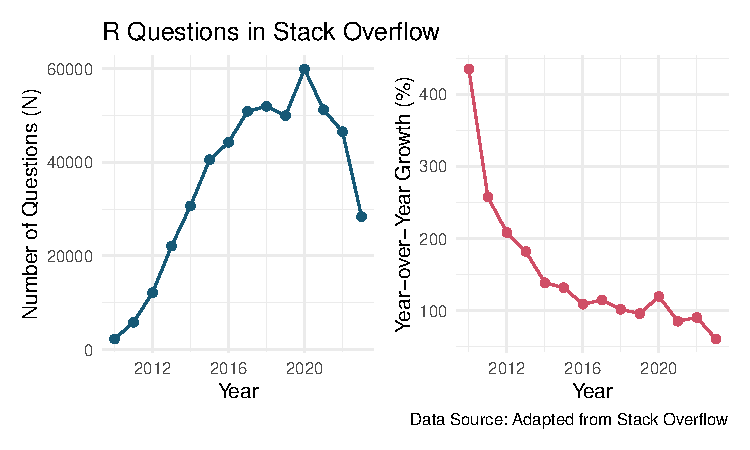
\includegraphics[keepaspectratio]{cpp11armadillo_files/figure-pdf/stackoverflow-1.pdf}}

}

\caption{R Questions in Stack Overflow increase from 2,260 in 2010 to
28,385 in 2023 with a peak of 59,895 in 2020.}

\end{figure}%

Large Language Model tools, including ChatGPT, explain a decline in the
popularity and the number of R questions in Stack Overflow and other
coding forums {[}11{]}. Another explanation in the decline in last years
in the plot is that already answered questions are not asked again, and
the community has access to existing answers through search engines.

\section{Software description}\label{software-description}

`cpp11armadillo' uses `cpp11' to leverage modern C++ features to provide
a seamless interface between R and the Armadillo library, offering
high-performance linear algebra operations with minimal overhead.

`cpp11' is a modern rewrite of the C++ interface for R, designed to
improve safety, performance, and ease of use. It enforces copy-on-write
semantics to prevent unintended modifications to data, ensuring that
changes to objects do not affect other references. `cpp11' provides
safer access to R's C API, reducing runtime errors in C++ code. It also
supports ALTREP objects for efficient memory management and deferred
computations, making it ideal for handling large datasets. By using
UTF-8 strings throughout, `cpp11' ensures robust handling of datasets
created in different countries where encodings vary {[}2{]}.

Built on C++11 features like smart pointers and lambdas, `cpp11' offers
a more straightforward and efficient implementation compared to `Rcpp'.
Its header-only design eliminates ABI compatibility issues, making it
easier to integrate and manage in projects. `cpp11' also compiles
faster, uses less memory, and grows vectors more efficiently, optimizing
performance when dealing with large amounts of data. These improvements
make `cpp11' a powerful, streamlined tool for developers who need
reliable, high-performance C++ bindings for R {[}2{]}.

`cpp11armadillo' offers vendoring, something not available in
`RcppArmadillo'. Vendoring is a well-known concept in the Go community,
and it consists in copying the dependency code directly into a project's
source tree. This approach ensures that dependencies remain fixed and
stable, preventing any external changes from inadvertently breaking the
project. While vendoring offers stability, it comes with trade-offs. The
primary advantage is that updates to the `cpp11armadillo' library will
not disrupt existing code, and it also copies `cpp11' C++ headers.
However, the drawbacks include an increase in package size and the loss
of automatic updates, meaning that bug fixes and new features will only
be available when manually updated.

Vendoring which can simplify the installation process and reduce
dependency issues, especially when working in environments with
restricted access to the Internet. For instance, the
\href{https://docs.scinet.utoronto.ca/index.php/Niagara_Quickstart}{Niagara
Supercomputer} that we use at the University of Toronto has restricted
access to the Internet, and vendoring can simplify the installation
process. In other words, vendoring allows the package creator to provide
a dependency-free package that can be installed in any environment
without requiring the end user to install `cpp11' nor `cpp11armadillo'.
This approach makes `cpp11armadillo' a dependency for the developer but
not for the end user.

\section{Software functionalities}\label{software-functionalities}

To use `cpp11armadillo', users must first install the package from CRAN
or GitHub. The package includes the Armadillo library, no additional
installation is required. The following code shows how to install the
package:

\begin{Shaded}
\begin{Highlighting}[]
\FunctionTok{install.packages}\NormalTok{(}\StringTok{"cpp11armadillo"}\NormalTok{)}

\CommentTok{\# or}
\NormalTok{remotes}\SpecialCharTok{::}\FunctionTok{install\_github}\NormalTok{(}\StringTok{"pachadotdev/cpp11armadillo"}\NormalTok{)}
\end{Highlighting}
\end{Shaded}

Once installed, users can use the provided package template function to
create a new package that uses C++ code with Armadillo. The package
template includes simple examples and all the necessary files to compile
the code and install the new R package. The following code shows how to
create a new package:

\begin{Shaded}
\begin{Highlighting}[]
\CommentTok{\# subdir + package name}
\CommentTok{\# subdir can be "." to create the package in the current directory}
\NormalTok{cpp11armadillo}\SpecialCharTok{::}\FunctionTok{pkg\_template}\NormalTok{(}\StringTok{"pkgtemplate"}\NormalTok{, }\StringTok{"myownpackage"}\NormalTok{)}
\end{Highlighting}
\end{Shaded}

Then the user can open a new RStudio session to modify the package
template, or type \texttt{setwd("pkgtemplate")} to open the package in
the current R session. We highly recommend that users start by reading
the readme file in the package template directory to understand the
package structure and the necessary steps to add functions and build the
package.

The package
\href{https://pacha.dev/cpp11armadillo/index.html}{vignettes} cover the
directories organization and the necessary steps to build an R package
with relatively low setup efforts.

It is important to note that `cpp11armadillo' only work within an R
package, and it is not possible to compile individual C++ scripts on the
fly. This design choice ensures that the R and C++ code is organized
following the organization described in {[}12{]}.

The package creator needs to export the functions for the end user. For
example, for the following C++ function:

\begin{Shaded}
\begin{Highlighting}[]
\DataTypeTok{double} \VariableTok{plus\_one\_}\OperatorTok{(}\AttributeTok{const} \DataTypeTok{double} \OperatorTok{\&}\NormalTok{x}\OperatorTok{)} \OperatorTok{\{}
  \ControlFlowTok{return}\NormalTok{ x }\OperatorTok{+} \DecValTok{1}\OperatorTok{;}
\OperatorTok{\}}
\end{Highlighting}
\end{Shaded}

The function must be exported and it can be documents in the R package
as follows:

\begin{Shaded}
\begin{Highlighting}[]
\CommentTok{\#\textquotesingle{} Add one to a number}
\CommentTok{\#\textquotesingle{} @param x A number}
\CommentTok{\#\textquotesingle{} @return The number plus one}
\CommentTok{\#\textquotesingle{} @export}
\NormalTok{plus\_one }\OtherTok{\textless{}{-}} \ControlFlowTok{function}\NormalTok{(x) \{}
  \FunctionTok{plus\_one\_}\NormalTok{(x)}
\NormalTok{\}}
\end{Highlighting}
\end{Shaded}

\section{Illustrative examples}\label{illustrative-examples}

In order to evaluate the performance of `cpp11armadillo', we compared it
with native R functions and `RcppArmadillo'. To provide a point of
reference, we also used `NumPy', a popular numerical computing library
for Python, which is known for its performance and ease of use. For all
the benchmarks, we used a value of \(n = 10,000\).

Compiling the benchmarking functions took 4 seconds using
`cpp11armadillo', and 9 seconds using RcppArmadillo. These functions are
quite simple, but this comparison is consistent with the build times for
general usage R packages, as shown in the following table:

\begin{longtable}[]{@{}lcc@{}}
\caption{Benchmark comparison of `cpp11' and `Rcpp'
{[}2{]}.}\tabularnewline
\toprule\noalign{}
Package & `cpp11' compile time & `Rcpp' compile time \\
\midrule\noalign{}
\endfirsthead
\toprule\noalign{}
Package & `cpp11' compile time & `Rcpp' compile time \\
\midrule\noalign{}
\endhead
\bottomrule\noalign{}
\endlastfoot
haven & 7.1s & 17.4s \\
readr & 81.0s & 124.1s \\
roxygen2 & 4.2s & 17.3s \\
tidyr & 3.3s & 14.3s \\
\end{longtable}

Table 1 reveals that R packages using `cpp11' compile faster than using
`Rcpp'. This is the result of a full refactor of the C++ parts of these
packages to use `cpp11' instead of `Rcpp' to expose C++ functions to R.

\subsection{Eigenvalues}\label{eigenvalues}

We focused on a single test consisting in obtaining the eigenvalues for
a dense (symmetric) matrix of size \(n \times n\).

The R code for the computation is as follows:

\begin{Shaded}
\begin{Highlighting}[]
\NormalTok{bench\_r }\OtherTok{\textless{}{-}} \ControlFlowTok{function}\NormalTok{(m) \{}
  \FunctionTok{eigen}\NormalTok{(m)}\SpecialCharTok{$}\NormalTok{values}
\NormalTok{\}}
\end{Highlighting}
\end{Shaded}

An equivalent C++ code is as follows:

\begin{Shaded}
\begin{Highlighting}[]
\NormalTok{doubles }\VariableTok{bench\_eig\_cpp11armadillo\_}\OperatorTok{(}\AttributeTok{const}\NormalTok{ doubles\_matrix}\OperatorTok{\textless{}\textgreater{}\&}\NormalTok{ m}\OperatorTok{)} \OperatorTok{\{}
\NormalTok{  mat M }\OperatorTok{=}\NormalTok{ as\_Mat}\OperatorTok{(}\NormalTok{m}\OperatorTok{);}
\NormalTok{  colvec Y }\OperatorTok{=}\NormalTok{ eig\_sym}\OperatorTok{(}\NormalTok{M}\OperatorTok{);}
  \ControlFlowTok{return}\NormalTok{ as\_doubles}\OperatorTok{(}\NormalTok{Y}\OperatorTok{);}
\OperatorTok{\}}
\end{Highlighting}
\end{Shaded}

The Python code to have a referential computation time is as follows:

\begin{Shaded}
\begin{Highlighting}[]
\KeywordTok{def}\NormalTok{ bench\_eigenvalues\_py(M):}
    \ControlFlowTok{return}\NormalTok{ np.linalg.eigvals(M)}
\end{Highlighting}
\end{Shaded}

`cpp11armadillo' has a speed-up relative to `RcppArmadillo' of
approximately 0.1 times and a speed-up relative to base R of
approximately 2.4 times. The following table shows the median execution
time for one hundred thousand runs of the three implementations compared
to `NumPy' in Python:

\begin{longtable}[]{@{}rrrr@{}}
\caption{Execution Time for the Eigenvalues Benchmark.}\tabularnewline
\toprule\noalign{}
`cpp11armadillo' & `RcppArmadillo' & Base R & NumPy (Python) \\
\midrule\noalign{}
\endfirsthead
\toprule\noalign{}
`cpp11armadillo' & `RcppArmadillo' & Base R & NumPy (Python) \\
\midrule\noalign{}
\endhead
\bottomrule\noalign{}
\endlastfoot
21.86 s & 22.1 s & 52.42 s & 109.56 s \\
\end{longtable}

Table 2 shows a tie between `cpp11armadillo' and `RcppArmadillo' in
terms of speed, and both are faster than base R and `NumPy'. For this
particular operation, the ranking is: (1) C++, (2) R, and (3) Python.

\subsection{Multi-operation
Expression}\label{multi-operation-expression}

We focused on a single test consisting in a multi-operation expression
that computes \(P^T Q^{-1} R\), where \(P\) is a vector of length \(n\),
\(Q\) is a diagonal square matrix of size \(n \times n\) filled with
random values, and \(R\) is a vector of length \(n\). This test was
adapted from the official Armadillo documentation {[}13{]}.

The R code for the computation is as follows:

\begin{Shaded}
\begin{Highlighting}[]
\NormalTok{bench\_r }\OtherTok{\textless{}{-}} \ControlFlowTok{function}\NormalTok{(p, q, r) \{}
  \FunctionTok{as.numeric}\NormalTok{(}\FunctionTok{t}\NormalTok{(p) }\SpecialCharTok{\%*\%} \FunctionTok{solve}\NormalTok{(}\FunctionTok{diag}\NormalTok{(q)) }\SpecialCharTok{\%*\%}\NormalTok{ r)}
\NormalTok{\}}
\end{Highlighting}
\end{Shaded}

An equivalent C++ code is as follows:

\begin{Shaded}
\begin{Highlighting}[]
\DataTypeTok{double} \VariableTok{bench\_cpp11armadillo\_}\OperatorTok{(}\AttributeTok{const}\NormalTok{ doubles }\OperatorTok{\&}\NormalTok{p}\OperatorTok{,} \AttributeTok{const}\NormalTok{ doubles }\OperatorTok{\&}\NormalTok{q}\OperatorTok{,}
                             \AttributeTok{const}\NormalTok{ doubles }\OperatorTok{\&}\NormalTok{r}\OperatorTok{)} \OperatorTok{\{}
\NormalTok{  colvec P }\OperatorTok{=}\NormalTok{ as\_Col}\OperatorTok{(}\NormalTok{p}\OperatorTok{)}
\NormalTok{  colvec Q }\OperatorTok{=}\NormalTok{ as\_Col}\OperatorTok{(}\NormalTok{q}\OperatorTok{)}
\NormalTok{  colvec R }\OperatorTok{=}\NormalTok{ as\_Col}\OperatorTok{(}\NormalTok{r}\OperatorTok{)}
  \ControlFlowTok{return}\NormalTok{ as\_scalar}\OperatorTok{(}\NormalTok{trans}\OperatorTok{(}\NormalTok{P}\OperatorTok{)} \OperatorTok{*}\NormalTok{ inv}\OperatorTok{(}\NormalTok{diagmat}\OperatorTok{(}\NormalTok{Q}\OperatorTok{))} \OperatorTok{*}\NormalTok{ R}\OperatorTok{);}
\OperatorTok{\}}
\end{Highlighting}
\end{Shaded}

The Python code to have a referential computation time is as follows:

\begin{Shaded}
\begin{Highlighting}[]
\KeywordTok{def}\NormalTok{ bench\_multi\_py(p, q, r):}
    \ControlFlowTok{return} \BuiltInTok{float}\NormalTok{(np.dot(np.dot(p.T, np.linalg.inv(np.diag(q))), r))}
\end{Highlighting}
\end{Shaded}

`cpp11armadillo' has a speed-up relative to `RcppArmadillo' of
approximately 1.7 times and a speed-up relative to base R of
approximately 140,000 times. The following table shows the median
execution time for one hundred thousand runs of the three
implementations compared to NumPy in Python:

\begin{longtable}[]{@{}rrrr@{}}
\caption{Execution Time for the Multi-operation Expression
Benchmark.}\tabularnewline
\toprule\noalign{}
`cpp11armadillo' & `RcppArmadillo' & `NumPy' (Python) & Base R \\
\midrule\noalign{}
\endfirsthead
\toprule\noalign{}
`cpp11armadillo' & `RcppArmadillo' & `NumPy' (Python) & Base R \\
\midrule\noalign{}
\endhead
\bottomrule\noalign{}
\endlastfoot
26.1 us & 45.44 us & 2.60 s & 3.75 s \\
\end{longtable}

Table 3, unlike Table 2, reveals a clear difference between C++
functions exposed to R using `cpp11' and `Rcpp'. The ranking is: (1)
`cpp11', (2) `Rcpp', (3) R, and (4) Python.

The benchmarks were run on the
\href{https://docs.scinet.utoronto.ca/index.php/Niagara_Quickstart}{Niagara
Supercomputer} at the University of Toronto using forty cores and R,
Python, and the Armadillo library compiled with the Intel MKL library,
and the benchmarks were run sequentially.

The benchmarks were intentionally run on the Niagara Supercomputer to
ensure an accurate and controlled benchmarking environment, free from
potential distortions caused by background processes like automatic
updates, antivirus scans, cloud synchronization, or internet browsing
that are common on regular laptops or desktops {[}14{]}. This setup
allows us to isolate the performance of the package itself without
interference.

It is worth noting that these benchmarks can be run on a regular laptop
because a dense matrix of double precision numbers of
\(10,000 \times 10,000\) uses 800 MB in RAM plus the extra memory for
processing.

The reason to use the median execution time is to provide a robust
measure of the execution time, and it is less sensitive to outliers and
the stored results show there is variation in the execution time for
repeated runs.

The benchmarks do not cover sparse matrices, which are covered with
examples in `cpp11armadillo' documentation and follow the same syntax as
dense matrices. The Armadillo library can solve large-scale linear
algebra problems efficiently. These functions can be used to solve
problems in areas such as machine learning, optimization, and scientific
computing that involve a matrix of, for example, \(10^6 \times 10^6\)
elements. However, sparse matrices should only be used when the matrix
is mostly empty in the sense that most of its entries are zero. For
sparse matrices, the Armadillo library provides functions to convert
between dense and sparse matrices, and the library documentation warns
that sparse data objects are lighter but use compression techniques that
can slow down the computation {[}15{]}.

\section{Impact}\label{impact}

Researchers can explore questions involving complex matrix operations or
large datasets that introduce significant bottlenecks in R, and our
alternative scales with relative ease, as we showed in our benchmarks
where we were able to run the same code in a server with minimal setup
efforts due to vendoring.

The improved computational efficiency facilitates simulation studies,
and users can test and implement advanced linear algebra algorithms that
export the results to R for posterior analysis and visualization, and
the package can be used without needing a separate C++ compilation step.

Our benchmarks demonstrate substantial speed improvements compared to
existing equivalent implementations, enabling researchers to test and
modify computations with large datasets without a significant
computational overhead.

The package structure reduces the complexity of extending R with C++,
allowing users to focus on writing linear algebra instead of compiler
configurations to write high-performance code.

The software supports a structured workflow for combining R scripts with
efficient underlying C++ computations, enhancing reproducibility in
computational research.

By design, `cpp11armadillo' eliminates much of the boilerplate coding
required for R and C++ integration, allowing users to focus on algorithm
design. The simplified usage, besides scaling, facilitates collaboration
between R users and C++ developers, promoting interdisciplinary work.

The package is ideal for scientists who rely on matrix-heavy
computations. It may interest users from disciplines like biology,
finance, and physics, where high-performance computation is highly
desirable.

Companies working with R for data analysis and simulation could
integrate the package into their pipelines, benefiting from faster
computations, and this is compatible with the Apache license, which
allows commercial use. By lowering barriers to high-performance R and
C++ integrations, the package could inspire startups focused on
domain-specific software solutions or consulting services based on
efficient computational methods.

\section{Conclusion}\label{conclusion}

`cpp11armadillo' provides a simple and efficient way to integrate C++
code with R, leveraging the `cpp11' package and the Armadillo library.
It simplifies the process of writing C++ code for R users, allowing them
to focus on the logic of the algorithm rather than the technical details
of the integration. It can help to solve performance bottlenecks in `R'
code by using the efficient linear algebra operations provided by
Armadillo in cases where vectorization is challenging.

\section{Acknowledgments}\label{acknowledgments}

We thank the reviewers for their valuable feedback and suggestions. We
also thank Professor Salma Emara who taught us C++ and clearly cares
about her students.

\section*{References}\label{references}
\addcontentsline{toc}{section}{References}

\phantomsection\label{refs}
\begin{CSLReferences}{0}{0}
\bibitem[\citeproctext]{ref-eddelbuettel2011}
\CSLLeftMargin{{[}1{]} }%
\CSLRightInline{\href{https://doi.org/10.18637/jss.v040.i08}{D.
Eddelbuettel, R. Francois, Journal of Statistical Software 40 (2011)
1--18}.}

\bibitem[\citeproctext]{ref-cpp11}
\CSLLeftMargin{{[}2{]} }%
\CSLRightInline{D. Vaughan, J. Hester, R. François,
\href{https://CRAN.R-project.org/package=cpp11}{{cpp11}: A {C++}11
Interface for {R}'s {C} Interface}, 2023.}

\bibitem[\citeproctext]{ref-sanderson2016}
\CSLLeftMargin{{[}3{]} }%
\CSLRightInline{\href{https://doi.org/10.21105/joss.00026}{C. Sanderson,
R. Curtin, Journal of Open Source Software 1 (2016) 26}.}

\bibitem[\citeproctext]{ref-eddelbuettel2014}
\CSLLeftMargin{{[}4{]} }%
\CSLRightInline{\href{https://doi.org/10.1016/j.csda.2013.02.005}{D.
Eddelbuettel, C. Sanderson, Computational Statistics \& Data Analysis 71
(2014) 1054--1063}.}

\bibitem[\citeproctext]{ref-wickham2019}
\CSLLeftMargin{{[}5{]} }%
\CSLRightInline{\href{https://doi.org/10.21105/joss.01686}{H. Wickham,
M. Averick, J. Bryan, W. Chang, L.D. McGowan, R. François, G. Grolemund,
A. Hayes, L. Henry, J. Hester, M. Kuhn, T.L. Pedersen, E. Miller, S.M.
Bache, K. Müller, J. Ooms, D. Robinson, D.P. Seidel, V. Spinu, K.
Takahashi, D. Vaughan, C. Wilke, K. Woo, H. Yutani, Journal of Open
Source Software 4 (2019) 1686}.}

\bibitem[\citeproctext]{ref-r2024}
\CSLLeftMargin{{[}6{]} }%
\CSLRightInline{R Core Team, \href{https://www.R-project.org/}{{R}: A
Language and Environment for Statistical Computing}, {R} Foundation for
Statistical Computing, Vienna, Austria, 2024.}

\bibitem[\citeproctext]{ref-stroustrup2012}
\CSLLeftMargin{{[}7{]} }%
\CSLRightInline{\href{https://isocpp.org/tour}{B. Stroustrup, (2012)}.}

\bibitem[\citeproctext]{ref-burns2011}
\CSLLeftMargin{{[}8{]} }%
\CSLRightInline{P. Burns, The {R} Inferno, Lulu, 2011.}

\bibitem[\citeproctext]{ref-rpostgres}
\CSLLeftMargin{{[}9{]} }%
\CSLRightInline{H. Wickham, J. Ooms, K. Müller,
\href{https://CRAN.R-project.org/package=RPostgres}{{rpostgres}: {C++}
Interface to PostgreSQL}, 2023.}

\bibitem[\citeproctext]{ref-stackoverflow2024}
\CSLLeftMargin{{[}10{]} }%
\CSLRightInline{\href{https://data.stackexchange.com/stackoverflow/query/new}{Stack
Overflow, (2024)}.}

\bibitem[\citeproctext]{ref-kabir2024}
\CSLLeftMargin{{[}11{]} }%
\CSLRightInline{\href{https://doi.org/10.1145/3613904.3642596}{S. Kabir,
D.N. Udo-Imeh, B. Kou, T. Zhang, in: Proceedings of the 2024 {CHI}
{Conference} on {Human} {Factors} in {Computing} {Systems}, Association
for Computing Machinery, New York, NY, USA, 2024, pp. 1--17}.}

\bibitem[\citeproctext]{ref-wickham2023}
\CSLLeftMargin{{[}12{]} }%
\CSLRightInline{H. Wickham, J. Bryan, R Packages, O'Reilly, 2023.}

\bibitem[\citeproctext]{ref-armadillo2024}
\CSLLeftMargin{{[}13{]} }%
\CSLRightInline{\href{https://arma.sourceforge.net/speed.html}{C.
Sanderson, (2024)}.}

\bibitem[\citeproctext]{ref-beyer2019}
\CSLLeftMargin{{[}14{]} }%
\CSLRightInline{\href{https://doi.org/10.1007/s10009-017-0469-y}{D.
Beyer, S. Löwe, P. Wendler, International Journal on Software Tools for
Technology Transfer 21 (2019) 1--29}.}

\bibitem[\citeproctext]{ref-sanderson2019}
\CSLLeftMargin{{[}15{]} }%
\CSLRightInline{C. Sanderson, R. Curtin, Mathematical and Computational
Applications 24 (2019) 70.}

\end{CSLReferences}

%% The Appendices part is started with the command \appendix;
%% appendix sections are then done as normal sections
%% \appendix

%% \section{}
%% \label{}

%% References:
%% If you have bibdatabase file and want bibtex to generate the
%% bibitems, please use
%%
\bibliographystyle{elsarticle-num} 
\bibliography{references}

\end{document}
\endinput
%%
%% End of file `SoftwareX_arti\documentclass[10pt]{softwarex}
